% Options for packages loaded elsewhere
\PassOptionsToPackage{unicode}{hyperref}
\PassOptionsToPackage{hyphens}{url}
\PassOptionsToPackage{dvipsnames,svgnames*,x11names*}{xcolor}
%
\documentclass[]{article}
\usepackage{lmodern}
\usepackage{amssymb,amsmath}
\usepackage{ifxetex,ifluatex}
\ifnum 0\ifxetex 1\fi\ifluatex 1\fi=0 % if pdftex
  \usepackage[T1]{fontenc}
  \usepackage[utf8]{inputenc}
  \usepackage{textcomp} % provide euro and other symbols
\else % if luatex or xetex
  \usepackage{unicode-math}
  \defaultfontfeatures{Scale=MatchLowercase}
  \defaultfontfeatures[\rmfamily]{Ligatures=TeX,Scale=1}
\fi
% Use upquote if available, for straight quotes in verbatim environments
\IfFileExists{upquote.sty}{\usepackage{upquote}}{}
\IfFileExists{microtype.sty}{% use microtype if available
  \usepackage[]{microtype}
  \UseMicrotypeSet[protrusion]{basicmath} % disable protrusion for tt fonts
}{}
\makeatletter
\@ifundefined{KOMAClassName}{% if non-KOMA class
  \IfFileExists{parskip.sty}{%
    \usepackage{parskip}
  }{% else
    \setlength{\parindent}{0pt}
    \setlength{\parskip}{6pt plus 2pt minus 1pt}}
}{% if KOMA class
  \KOMAoptions{parskip=half}}
\makeatother
\usepackage{xcolor}\pagecolor[RGB]{28,30,38} \color[RGB]{213,216,218}
\IfFileExists{xurl.sty}{\usepackage{xurl}}{} % add URL line breaks if available
\IfFileExists{bookmark.sty}{\usepackage{bookmark}}{\usepackage{hyperref}}
\hypersetup{
  pdftitle={Fourier Analysis and the Theory of Distributions},
  pdfauthor={Kexing Ying},
  colorlinks=true,
  linkcolor=Maroon,
  filecolor=Maroon,
  citecolor=Blue,
  urlcolor=red,
  pdfcreator={LaTeX via pandoc}}
\urlstyle{same} % disable monospaced font for URLs
\usepackage[margin = 1.5in]{geometry}
\usepackage{graphicx}
\makeatletter
\def\maxwidth{\ifdim\Gin@nat@width>\linewidth\linewidth\else\Gin@nat@width\fi}
\def\maxheight{\ifdim\Gin@nat@height>\textheight\textheight\else\Gin@nat@height\fi}
\makeatother
% Scale images if necessary, so that they will not overflow the page
% margins by default, and it is still possible to overwrite the defaults
% using explicit options in \includegraphics[width, height, ...]{}
\setkeys{Gin}{width=\maxwidth,height=\maxheight,keepaspectratio}
% Set default figure placement to htbp
\makeatletter
\def\fps@figure{htbp}
\makeatother
\setlength{\emergencystretch}{3em} % prevent overfull lines
\providecommand{\tightlist}{%
  \setlength{\itemsep}{0pt}\setlength{\parskip}{0pt}}
\setcounter{secnumdepth}{5}
\usepackage{tikz}
\usepackage{physics}
\usepackage{amsthm}
\usepackage{mathtools}
\usepackage{esint}
\usepackage[ruled,vlined]{algorithm2e}

\usepackage{pgfplots}
\pgfplotsset{width=8cm,compat=1.9}

\theoremstyle{definition}
\newtheorem{theorem}{Theorem}
\newtheorem{definition*}{Definition}
\newtheorem{prop}{Proposition}
\newtheorem{corollary}{Corollary}[theorem]
\newtheorem*{remark}{Remark}
\theoremstyle{definition}
\newtheorem{definition}{Definition}[section]
\newtheorem{lemma}{Lemma}[section]
\newtheorem{proposition}{Proposition}[section]
\newtheorem{example}{Example}[section]
\newcommand{\diag}{\mathop{\mathrm{diag}}}
\newcommand{\Arg}{\mathop{\mathrm{Arg}}}
\newcommand{\hess}{\mathop{\mathrm{Hess}}}

\title{Fourier Analysis and the Theory of Distributions}
\author{Kexing Ying}

\begin{document}
\maketitle

{
\hypersetup{linkcolor=}
\setcounter{tocdepth}{2}
\tableofcontents
}
\newpage

\section{Orthonormal System}

We will in this section recall some results about orthonormal systems in Euclidean 
spaces\footnote{In this course, we shall call real inner product spaces Euclidean 
spaces.} and generalize them to complex spaces. 

\subsection{Euclidean Space}

\begin{definition}
  A system of nonzero vectors \(\{X_\alpha\} \subseteq R\) where \(R\) is an 
  Euclidean space is called orthogonal if \(\langle X_\alpha, X_\beta\rangle = 0\)
  for all \(\alpha \neq \beta\). 

  In addition, if for all \(\alpha\), \(\langle X_\alpha, X_\alpha\rangle = 1\), 
  we say the system is orthonormal.
\end{definition}

Clearly, given an orthogonal system \(\{X_\alpha\}\), we may normalize the vector 
such that \(\{X_\alpha / \|X_\alpha\|\}\) is an orthonormal system. Furthermore, 
recall that a system of orthogonal vectors is linearly independent.

\begin{definition}
  A complete (i.e. the smallest closed subspace containing the system is \(R\)) 
  orthogonal system \(\{X_\alpha\} \subseteq R\) is said to 
  be an orthogonal basis of \(R\). 
\end{definition}

Some important spaces we shall study in this course include \(\mathbb{R}^2\) 
(equipped with the Euclidean norm), \(l_2\), \(\mathcal{C}([-\pi , \pi])\) 
(the space of continuous functions on \([-\pi, \pi]\) equipped with the \(L_2\) norm). 

\begin{proposition}
  Let \(R\) be a separable Euclidean space. Then any orthogonal system in \(R\) 
  is countable. 
\end{proposition}
\begin{proof}
  By normalizing, we may assume the system \(\{X_\alpha\}\) is orthonormal. Then, 
  for \(\alpha \neq \beta\),
  \[\|X_\alpha - X_\beta\|^2 = \|X_\alpha\|^2 - 2\langle X_\alpha, X_\beta\rangle + 
  \|X_\beta\|^2 = \|X_\alpha\|^2 + \|X_\beta\|^2 = 2.\]
  Then, \(B_{1 / 2}(X_\alpha) \cap B_{1 / 2}(X_\beta) = \varnothing\) for all 
  \(\alpha \neq \beta\). Thus, if the system is not countable, we have found 
  a uncountable number of disjoint open balls, contradicting the separability of 
  \(R\).
\end{proof}

\begin{proposition}
  Let \(f_1, f_2, \cdots\) be a linearly independent system in a Euclidean space 
  \(R\). Then, there exists an orthonormal system \(\phi_1, \phi_2, \cdots\) such 
  that 
  \[\phi_n = a_{n_1} f_1 + \cdots + a_{n_n} f_n\]
  and 
  \[f_n = b_{n_1}\phi_1 + \cdots + b_{n_n} \phi_n\]
  for some \(a_{n_k}, b_{n_k} \in \mathbb{R}\) and \(a_{n_n}, b_{n_n} \neq 0\).
  Furthermore, the system \(\phi_1, \phi_2, \cdots\) is uniquely determined up 
  to a multiplication by \(\pm 1\).
\end{proposition}
\begin{proof}
  Use Gram-Schmidt. 
\end{proof}

\begin{corollary}
  A separable Euclidean space \(R\) possesses an orthonormal basis.
\end{corollary}
\begin{proof}
  Simply obtain the orthonormal system corresponding to the countable dense 
  system of \(R\). The resulting system is complete since the two systems have the 
  same linear closure.
\end{proof}

\begin{definition}[Fourier Coefficients]
  Let \(\phi_1, \phi_2, \cdots\) be an orthonormal system in \(R\) and let \(f \in R\). 
  Consider the sequence \(c_k = \langle f, \phi_k \rangle\) for all \(k = 1, 2, \cdots\). 
  Then \(c_k\) are called the coordinates or Fourier coefficients of \(f\) with respect 
  to the system \(\{\phi_k\}\) and \(\sum_{k = 1}^\infty c_k \phi_k\) is 
  called the Fourier series of \(f\).
  
  Note that this series in the definition is a formal series as we do not yet 
  know whether or not the series converges.
\end{definition}

In the finite case, it is not difficult to see that the sequence 
\(\alpha_k\) for \(k = 1, \cdots, n\) which minimizes \(\|f - S_n^{(\alpha)}\|\) 
where \(S_n^{(\alpha)} := \sum_{k = 1}^n \alpha_k \phi_k\) is the Fourier coefficients. 
Indeed, we have 
\[\begin{split}
  \|f - S_n^{(\alpha)}\|^2 & = \langle f, f \rangle - 2 \langle f, S_n^{(\alpha)} \rangle +
    \langle S_n^{(\alpha)}, S_n^{(\alpha)} \rangle\\
    & = \|f\|^2 - 2 \sum \alpha_k c_k + \sum \alpha_k^2\\
    & = \|f\|^2 - \sum c_k^2 + \sum (\alpha_k - c_k)^2.
\end{split}\]
Hence, \(\|f - S_n^{(\alpha)}\|\) is minimized when \(\alpha_k = c_k\) for all 
\(k = 1, \cdots, n\). With this in mind, choosing \(\alpha\) to be the Fourier 
coefficients, we have 
\[\|f - S_n^{(c)}\| = \|f\|^2 - \sum_{k = 1}^n c_k^2.\]
Geometrically, \(f - S_n^{(\alpha)}\) is orthogonal to the subspace generated by 
\(\phi_1, \cdots, \phi_n\) if and only if \(\alpha = c\).

Furthermore, by noting \(0 \le \|f - S_n^{(c)}\| = \|f\|^2 - \sum_{k = 1}^n c_k^2\), 
we have 
\[\sum_{k = 1}^n c_k^2 \le \|f\|^2 < \infty,\]
and hence, taking \(n \to \infty\), we have \(\sum_{k = 1}^\infty c_k^2\) exists 
and is bounded above by \(\|f\|^2\). This inequality is known as the Bessel inequality.

\begin{definition}[Closed Orthonormal System]
  The orthonormal system \(\{\phi_k\}\) is closed if for any \(f \in R\), we have 
  \[\sum_{k = 1}^\infty c_k^2 = \|f\|^2.\]
  This property is called the Parseval equality.
\end{definition}

Again, by observing \(\|f - S_n^{(c)}\| = \|f\|^2 - \sum_{k = 1}^n c_k^2\),
the system is closed if and only if for any \(f\), the partial sums of the 
Fourier series converge to \(f\), i.e. \(f = \sum_{k = 1}^\infty c_k \phi_k\).

\begin{proposition}
  In a separable Euclidean space \(R\), an orthonormal system is complete 
  if and only if it is closed.
\end{proposition}
\begin{proof}
  Suppose first that \(\{\phi_k\}\) is closed. Then, for all \(f \in R\), 
  \(f = \sum_{k = 1}^\infty c_k \phi_k\). Thus, the finite linear combinations of 
  \(\{\phi_k\}\) is dense in \(R\) and thus, \(\{\phi_k\}\) is complete.

  On the other hand, suppose that \(\{\phi_k\}\) is complete (it is countable 
  as \(R\) is separable), for any \(f \in R\), there exists some \(\alpha^k\) 
  such that \(\|f - S^{(\alpha^k)}_\infty\| \to 0\). As we have seen, for any partial 
  sum \(S^{(\alpha^k)}_n\), we have \(\|f - S^{(c)}_n\| \le \|f - S^{(\alpha^k)}_n\|\) 
  and so, 
  \[\|f - S^{(c)}_\infty\| \le \|f - S^{(\alpha^k)}_\infty\| \to 0\]
  implying \(\|f - S^{(c)}_\infty\| = 0\) and the system is closed.
\end{proof}


\begin{proposition}
  Given \(f, g \in R\) and a closed orthonormal system \(\{\phi_k\}\), 
  \[\langle f, g \rangle = \sum_{k = 1}^\infty c_k d_k\]
  where \((c_k), (d_k)\) are the Fourier coefficients of \(f\) and \(g\) with respect 
  to \(\{\phi_k\}\) respectively.
\end{proposition}
\begin{proof}
  We have, by Parseval's identity, \(\|f\|^2 = \sum c_k^2\), \(\|g\|^2 = \sum d_k^2\) 
  and \(\|f + g\|^2 = \sum (c_k + d_k)^2 = \sum c_k^2 + 2 \sum c_k d_k + \sum d_k^2\),
  we have 
  \[\sum c_k^2 + 2 \sum c_k d_k + \sum d_k^2 = \|f + g\|^2 = \|f\|^2 + 2\langle f, g\rangle + \|g\|^2.\]
  Thus, cancelling using \(\|f\|^2 = \sum c_k^2\) and \(\|g\|^2 = \sum d_k^2\), we have 
  \(\langle f, g \rangle = \sum_{k = 1}^\infty c_k d_k\) as required.
\end{proof}

In the case the system is only orthogonal but not necessary orthonormal, we may 
normalize the Fourier coefficients, i.e. given an orthogonal system \(\{\phi_k\}\), 
we have \(\{\phi / \|\phi_k\|\}\) is an orthonormal system, and so, we define
\[c_k = \left\langle f, \frac{\phi_k}{\|\phi_k\|} \right\rangle = \frac{1}{\|\phi_k\|} \langle f, \phi_k \rangle.\]
Similarly, the Fourier series of \(f\) is becomes 
\[\sum_{k = 1}^\infty c_k \frac{\phi_k}{\|\phi_k\|} = \sum \frac{\langle f, \phi_k\rangle}{\|\phi_k\|^2} \phi_k.\]
Substituting this definition of the Fourier coefficients into the Bessel inequality,
we obtain 
\[\sum_{k = 1}^\infty \frac{\langle f, \phi_k\rangle^2}{\|\phi_k\|^2} \le \|f\|^2,\]
for any orthogonal system \(\{\phi_k\}\).

\begin{theorem}[Riesz]
  Let \(\{\phi_k\}\) be a orthonormal system in a complete Euclidean space \(R\) 
  (i.e. a real Hilbert space) and let \(c \in \ell_2\) 
  (i.e. \(\sum_{k = 1}^\infty c_k^2 < \infty\)). Then, 
  there exists some \(f \in R\) such that \(c_k = \langle f, \phi_k \rangle\) and 
  Parseval's identity holds, i.e.
  \[\sum_{k = 1}^\infty c_k^2 = \|f\|^2.\]
\end{theorem}
\begin{proof}
  Let \(f_n := \sum_{k = 1}^n c_k \phi_k\). Then, by definition, we have 
  \(c_k = \langle f_n, \phi_k \rangle\) for all \(k = 1, \cdots, n\). Then, 
  for all \(p \ge 1\), we have
  \[\|f_{n + p} - f_n\|^2 = \|c_{n + 1} \phi_{n + 1} + \cdots + c_{n + p} \phi_{n + p}\|^2 
    = \sum_{k = n + 1}^{n + p} c_k^2.\]
  Now, as \(\sum c_k^2 < \infty\), we have \(\{f_n\}\) is Cauchy, and thus, as 
  \(R\) is complete, there exists some \(f \in R\) such that \(f_n \to f\). 
  Thus, by noting, 
  \[\langle f, \phi_k \rangle = \langle f_n \phi_k\rangle + \langle f - f_n, \phi_k\rangle
    = c_k + \langle f - f_n, \phi_k\rangle,\]
  where \(\langle f - f_n, \phi_k\rangle \to 0\) as \(n \to \infty\) since 
  \(|\langle f - f_n, \phi_k\rangle| \le \|f - f_n\| \|\phi_k\|\) by the 
  Cauchy-Schwarz inequality, we have \(c_k = \langle f, \phi_k\rangle\).

  Finally, Parseval's identity, follows as \(\|\cdot\|^2\) is continuous in a 
  normed space.
\end{proof}

Let us recall the following result from functional analysis.

\begin{proposition}
  Any separable Hilbert space is isomorphic to \(\ell_2\) (thus, any two separable 
  Hilbert spaces are isomorphic). 
\end{proposition}
\begin{proof}
  Let \(H\) be a separable Hilbert space and choose \(\{\phi_k\}\) a complete 
  orthonormal system (which exists as \(H\) is separable). Then, for any \(f \in H\), 
  we map \(f\) to the sequence corresponding to its Fourier coefficients, i.e.
  \[\psi : f \mapsto (c_1, c_2, \cdots)\]
  which is well-defined by Bessel's inequality. On the other hand, by Riesz's 
  theorem, for any \(x \in \ell_2\), \(\sum x_k^2 < \infty\) and so, there 
  exists a unique \(f \in H\),  such that \(\psi(f) = x\). Thus, as \(\psi\) is 
  clearly linear (as the inner products are linear with respect to the left 
  component), we have the isomorphism between \(H\) and \(\ell_2\).
\end{proof}

\subsection{Complex Inner Product Space}

We will in the course take the complex inner product to be anti-linear in the 
second component. As promised earlier, most definitions can be generalized 
from the real case to the complex directly.

\begin{definition}[Fourier Coefficients]
  Let \(R\) be a complex inner product space. Then, for an orthonormal system 
  \((\phi_n)\) and \(f \in R\), we define its Fourier coefficients to be 
  \(c_k := \langle f, \phi_k\rangle\) for all \(k = 1, \cdots, n\). Similarly,
  we define the Fourier series of \(f\) to be the formal series 
  \(\sum_{k = 1}^\infty c_k \phi_k\).
\end{definition}

Going through the same argument as the real case, we obtain the complex version 
of Bessel's inequality.

\begin{proposition}[Bessel's Inequality]
  Given an orthonormal system \((\phi_n)\) and \(f \in R\), we have 
  \[\sum_{k = 1}^\infty |c_k|^2 \le \|f\|^2.\]
\end{proposition}

Going through all proved theorems for real spaces, we find they also hold for 
complex spaces (with trivial modifications).

\newpage
\section{Trigonometric Series}

We will consider the space \(L_2[-\pi, \pi]\) (the space of square-integrable functions 
from \([-\pi, \pi]\) quotiented by the a.e.-equal equivalence relation equipped with 
the inner product \(\langle f, g\rangle := \int_{[-\pi, \pi]} fg \dd\lambda\)), and the 
trigonometric system 
\[\{\mathbf{1}, \cos(n x), \sin(n x) \mid n = 1, 2, \cdots\}.\]
It is not difficult to see that this system is orthogonal, but in fact, it is 
also complete. Indeed, completeness follows by the Weierstrass approximation theorem 
for trigonometric polynomials (we will discuss this later / recall the Stone-Weierstrass 
theorem and observe that the trigonometric system seperates points).

Nonetheless, this system is not orthonormal, and thus, we normalise the system 
such that the system becomes 
\[\left\{\frac{1}{\sqrt{2\pi}}\mathbf{1}, \frac{1}{\sqrt{\pi}}\cos(n x), \frac{1}{\sqrt{\pi}}\sin(n x) \mid n = 1, 2, \cdots\right\}.\]
Hence, the Fourier series of an element \(f \in L_2[-\pi, \pi]\) becomes the 
famous formula
\[\frac{a_0}{2} + \sum_{k = 1}^\infty (a_k \cos kx + b_k \sin k x),\]
where 
\[a_k := \frac{1}{\pi}\int_{[-\pi, \pi]} f(x) \cos(k x) \lambda(\dd x),
  b_k := \frac{1}{\pi}\int_{[-\pi, \pi]} f(x) \sin(k x) \lambda(\dd x).\]
By recalling the above theory, the \(n\)-th partial sum of this series provides the best 
(in \(L_2\) metric) approximation of \(f\) among all trigonometric polynomials 
of degree \(n\). Hence, as the trigonometric system is complete, Parseval's 
identity holds, and so, 
\[\|f - S_n\|_2 \to 0, \text{ as } n \to \infty.\]
By observing that \(e^{ix} = \cos x + i\sin x\), we may rewrite the Fourier series 
can be written in the complex form. In particular, \(L_2[-\pi, \pi]\) has the 
orthogonal system \(\{e^{inx} \mid n \in \mathbb{Z}\}\) and the Fourier series 
of \(f \in L_2[-\pi, \pi]\) is given by 
\[\sum_{n = -\infty}^\infty c_n e^{inx}, \text{ where }
  c_n = \frac{1}{2\pi} \int_{[-\pi, \pi]} f(x)e^{-inx}\lambda(\dd x).\]
\begin{itemize}
  \item Since a function on \([-\pi, \pi]\) can be extended to \(\mathbb{R}\) by periodicity, 
    we can, instead of functions on \([-\pi, \pi]\) consider periodic functions with 
    period \(2\pi\) on \(\mathbb{R}\).
  \item Since \(\cos nx, \sin nx\) are bounded functions, the integrals defining 
    the trigonometric Fourier coefficients exists for any function in \(L_1[-\pi, \pi]\), 
    i.e. if \(f \in L_1[-\pi, \pi]\), then 
    \[\int f \cos(nx), \int f\sin(nx) < \int |f| < \infty.\]
  \item \(L_2[-\pi, \pi] \subseteq L_1[-\pi, \pi]\) by Hölder's inequality and thus,
    with the above remark in mind, the definition of Fourier series is also well-defined 
    for any integrable functions (though convergence is much opaque in this case).
\end{itemize}
While the Fourier series of \(f\) converges to \(f\) in \(L_2\) though it 
is not clear that the Fourier series converges point-wise to \(f\) 
(it might be interesting to recall that convergence in \(L_p\) implies convergence 
in measure and the existence of a subsequence which converges almost everywhere).  

Consider the partial sum of the Fourier series of \(f \in L_2[-\pi, \pi]\),
\[\begin{split}
  S_n(x) & = \frac{a_0}{2} + \sum_{k = 1}^n (a_k \cos kx + b_k \sin kx)\\
  & = \frac{1}{\pi}{\int_{[-\pi, \pi]} f(t)}\left(\frac{1}{2} + \sum_{k = 1}^n 
    (\cos kx \cos kt + \sin kx \sin kt)\right)\lambda(\dd t)\\
  & = \frac{1}{\pi}{\int_{[-\pi, \pi]} f(t)}\left(\frac{1}{2} + \sum_{k = 1}^n 
  \cos k(t - x)\right)\lambda(\dd t).
\end{split}\]
By noting the identity
\[\frac{1}{2} + \sum_{k = 1}^n \cos ku = \frac{\sin \frac{2n + 1}{2}u}{2\sin \frac{u}{2}},\]
we obtain 
\[S_n(x) = \frac{1}{\pi}{\int_{[-\pi, \pi]} f(t)} 
  \frac{\sin \frac{2n + 1}{2}(t - x)}{2\sin \frac{t - x}{2}} \lambda(\dd t).\]
Finally, by noting the periodicity of \(f\), by change of variable \(z = t - x\),
we obtain 
\[S_n(x) = \int_{[-\pi, \pi]} f(x + z) D_n(z) \lambda(\dd z), \text{ where }
  D_n(z) := \frac{1}{2\pi} \frac{\sin \frac{2n + 1}{2}z}{\sin \frac{z}{2}}\]
and \(D_n\) is known as the Dirichlet kernel. We remark that the Dirichlet kernel 
\(D_n(z)\) tends to \(\frac{2n + 1}{2\pi}\) as \(z \to 0\) and rapidly osculates 
for large \(n\) though this does not impact our calculation as we are dealing 
with a point which has measure 0. 

\begin{center}
  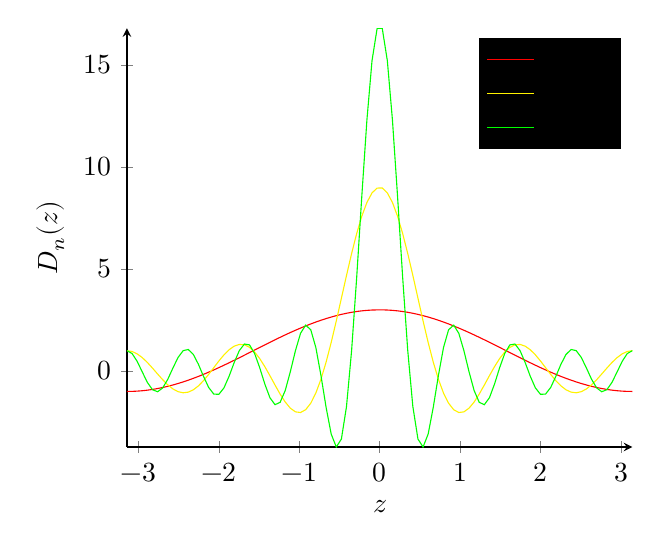
\begin{tikzpicture}
    \begin{axis}[
        legend style={fill=black,draw=white},
        axis lines = left,
        xlabel = \(z\),
        ylabel = {\(D_n(z)\)},
    ]
    %Below the red parabola is defined
    \addplot [
        domain=-pi:pi, 
        samples=100, 
        color=red,
    ]
    {sin(deg((3 / 2) * x)) / sin(deg(x / 2))};
    \addlegendentry{\(n = 1\)}
    %Here the blue parabola is defined
    \addplot [
        domain=-pi:pi, 
        samples=100, 
        color=yellow,
    ]
    {sin(deg((9 / 2) * x)) / sin(deg(x / 2))};    
    \addlegendentry{\(n = 4\)}
    \addplot [
        domain=-pi:pi, 
        samples=100, 
        color=green,
    ]
    {sin(deg((17 / 2) * x)) / sin(deg(x / 2))};    
    \addlegendentry{\(n = 8\)}
  \end{axis}
  \end{tikzpicture}
\end{center}

By observing the graph of the Dirichlet kernel, in some heuristic sense, we note that 
\(D_n(z) \to \delta(z)\) for some function where \(\delta\) is 0 at all points but 
\(z = 0\) while \(\int_{[-\epsilon, \epsilon]} \delta \dd \lambda = 1\) for all 
\(\epsilon > 0\). Such an function cannot exist, however it motivates the second 
part of the course - the theory of distributions.

\subsection{Conditions for Point-wise Convergence}

We observe that \(\|D_n\|_1 = 1\) and so we may write 
\[S_n(x) - f(x) = \int_{[-\pi, \pi]} (f(x + z) - f(x)) D_n(z) \lambda(\dd z).\]
Clearly, \(S_n(x) \to f(x)\) as \(n \to \infty\) if and only if the right hand side
of the above tends to 0. 

\begin{lemma}[Riemann-Lebesgue]
  If \(\phi \in L_1[a, b]\) for some \(a < b\), then both
  \[\int_{[a, b]} \phi(x)\sin (\gamma x) \lambda(\dd x), 
    \int_{[a, b]} \phi(x)\cos (\gamma x) \lambda(\dd x)\]
  tends to 0 as \(\gamma \to \infty\).
\end{lemma}
\begin{proof}
  We will prove the statement for the \(\sin\) case. We observe that if 
  \(\phi\) is continuously differentiable, by integration by parts, we have 
  \[\int_{[a, b]} \phi(x)\sin (\gamma x) \lambda(\dd x) = 
    \left[-\phi(x)\frac{\cos\gamma x}{\gamma}\right]^b_a + 
    \int_{[a, b]} \phi'(x) \frac{\cos \gamma x}{\gamma} \lambda(\dd x),\]
  which tends to 0 as \(\gamma \to \infty\) (we note that \(\phi'\) is continuous 
  on a compact set, and hence bounded above). Now, in the general case, we observe 
  that continuously differentiable functions are everywhere dense in \(L_1[a, b]\), 
  and so, for every \(\epsilon > 0\), there exists some continuously differentiable 
  \(\phi_\epsilon(x)\), such that 
  \[\int_{[a, b]} |\phi - \phi_\epsilon| \dd \lambda = \|\phi - \phi_\epsilon\|_1 < \frac{\epsilon}{2}.\]
  Hence, 
  \[\begin{split}
    \left|\int_{[a, b]} \phi(x) \sin(\gamma x) \lambda(\dd x)\right| 
    & \le \left|\int_{[a, b]} (\phi(x) - \phi_\epsilon(x)) \sin(\gamma x) \lambda(\dd x)\right| 
      + \left| \int_{[a, b]} \phi_\epsilon(x) \sin(\gamma x) \lambda(\dd x)\right|\\
    & \le \|\phi - \phi_\epsilon\|_1 + \left| \int_{[a, b]} \phi_\epsilon(x) \sin(\gamma x) \lambda(\dd x)\right|\\
    & < \frac{\epsilon}{2} + 
    \left| \int_{[a, b]} \phi_\epsilon(x) \sin(\gamma x) \lambda(\dd x)\right|.
  \end{split}\]
  Since \(\phi_\epsilon\) is continuously differentiable, the last term tends to 
  0 as \(\gamma \to \infty\) implying it is less than \(\epsilon / 2\) for sufficiently 
  large \(\gamma\). Thus, we have established the required limit. 
\end{proof}

\begin{corollary}
  If \(f \in L_1[-\pi, \pi]\), then, its Fourier coefficients \(a_k, b_k \to 0\) 
  as \(k \to \infty\).
\end{corollary}

With the above in mind, we will now provide a sufficient condition for convergence of 
Fourier series at a point \(x\).

\begin{theorem}
  If \(f \in L_1[-\pi, \pi]\) and for any \(x \in [-\pi, \pi]\), \(\delta > 0\), 
  \[\int_{[-\delta, \delta]} \left|\frac{f(x + t) - f(t)}{t}\right| \lambda(\dd t) < \infty\]
  exists (this is called Dini's condition), then \(S_n(x) \to f(x)\) as \(n \to \infty\).
\end{theorem}
\begin{proof}
  We observe
  \[\begin{split}
    S_n(x) - f(x) & = \int_{[-\pi, \pi]} (f(x + z) - f(x)) D_n(z) \lambda(\dd z)\\
    & = \frac{1}{2\pi}\int_{[-\pi, \pi]} \frac{f(x + z) - f(x)}{z} 
      \frac{z}{\sin \frac{z}{2}} \sin \left(\frac{2 n + 1}{2}z\right)\lambda(\dd z).\\
  \end{split}\]
  Then, if Dini's condition is satisfied, as \(\sin \frac{z}{2}\) is bounded on 
  \([-\pi, \pi]\), we have 
  \[\frac{f(x + z) - f(x)}{z} \frac{z}{\sin \frac{z}{2}} \in L_1[-\pi, \pi]\]
  and hence, by the Riemann-Lebesgue lemma, \(S_n(x) - f(x) \to 0\) as 
  \(n \to \infty\).
\end{proof}

We observe an trivial sufficient condition for which Dini's condition holds. 
In particular, the Dini condition holds if \(f\) is continuous at \(x\) and its derivative at 
\(x\) exists (or the limit of the derivative exists from the right and the left).

Suppose on the other hand that \(f\) has a discontinuity of the first kind at 
\(x\) (i.e. both the limit from the left and the right exists at \(x\)). Then, 
the argument in the proof remains to hold if we replace the Dini condition by 
\[\int_{[-\delta, 0] } \left|\frac{f(x + t) - f(t)}{t}\right| \lambda(\dd t) < \infty
\text{ and } 
\int_{[0, \delta] } \left|\frac{f(x + t) - f(t)}{t}\right| \lambda(\dd t) < \infty.\]
Then, denoting \(f(x + 0), f(x - 0)\) the limit of \(f\) at \(x\) from the right and the 
left respectively, we have
\[\begin{split}
  &S_n(x) - \frac{f(x + 0) + f(x - 0)}{2} =\\ 
  &\int_{[-\pi, 0]} (f(x + z) - f(x - 0)) D_n(z) \lambda(\dd z)
 + \int_{[0, \pi]} (f(x + z) - f(x + 0)) D_n(z) \lambda(\dd z)
 \end{split}\]
Hence, the \(S_n(x)\) converges to the average of the limit \(f\) at \(x\) from 
the left and from the right.

Let us summarise the above in the following statement.

\begin{proposition}
  If \(f\) is a bounded function of period \(2\pi\) with only 
  discontinuities of the first kind, and also possesses at each point left and right 
  derivatives, Then, its Fourier series converges everywhere and its sum equals 
  \(f(x)\) at points of continuity and equals 
  \[\frac{f(x + 0) + f(x - 0)}{2}\]
  at points of discontinuity.
\end{proposition}

We remark there exists continuous functions whose Fourier series diverge at some 
points. More curiously, there exists \(L_1\) functions which diverge at all points.

\end{document}